\chapter{Chemisch evenwicht: quotiënt en constante}\label{ch:g12:equilibrium}

Een dichte fles bruisend water houdt maandenlang zijn prik; open verliest
ze die in een middag. In geen van beide gevallen is er iets misgegaan. In
de dichte fles verlaat koolstofdioxide het water en keert het terug met
dezelfde snelheid, en de samenstelling blijft gelijk; draai de dop eraf,
en het gas dat ontsnapt, komt niet meer terug. Veel reacties gedragen zich
zo: ze stoppen voordat een \omterm{def:g7:chemical-reactions:reactant}{beginstof} op is, bij een evenwicht tussen twee
tegengestelde reacties. Dit hoofdstuk beschrijft dat evenwicht met één
getal.

\begin{recall}
De \omterm{def:g10:reaction-progress-table:extent}{reactievoortgang} $x$ van een reactie, haar maximum $x_{\max}$, en de
\omterm{def:g10:reaction-progress-table:limiting}{aflopende reacties} die dat bereiken (\cref{ch:g10:reaction-progress-table}).
Snelheden en \omterm{def:g12:reaction-rates:kinetic-factor}{kinetische factoren} (\cref{ch:g12:reaction-rates}); een
\omterm{def:g12:catalysis:catalyst}{katalysator} verandert de \omterm{def:g10:reaction-progress-table:system}{eindtoestand} niet (\cref{ch:g12:catalysis}).
\end{recall}

\begin{omfigure}
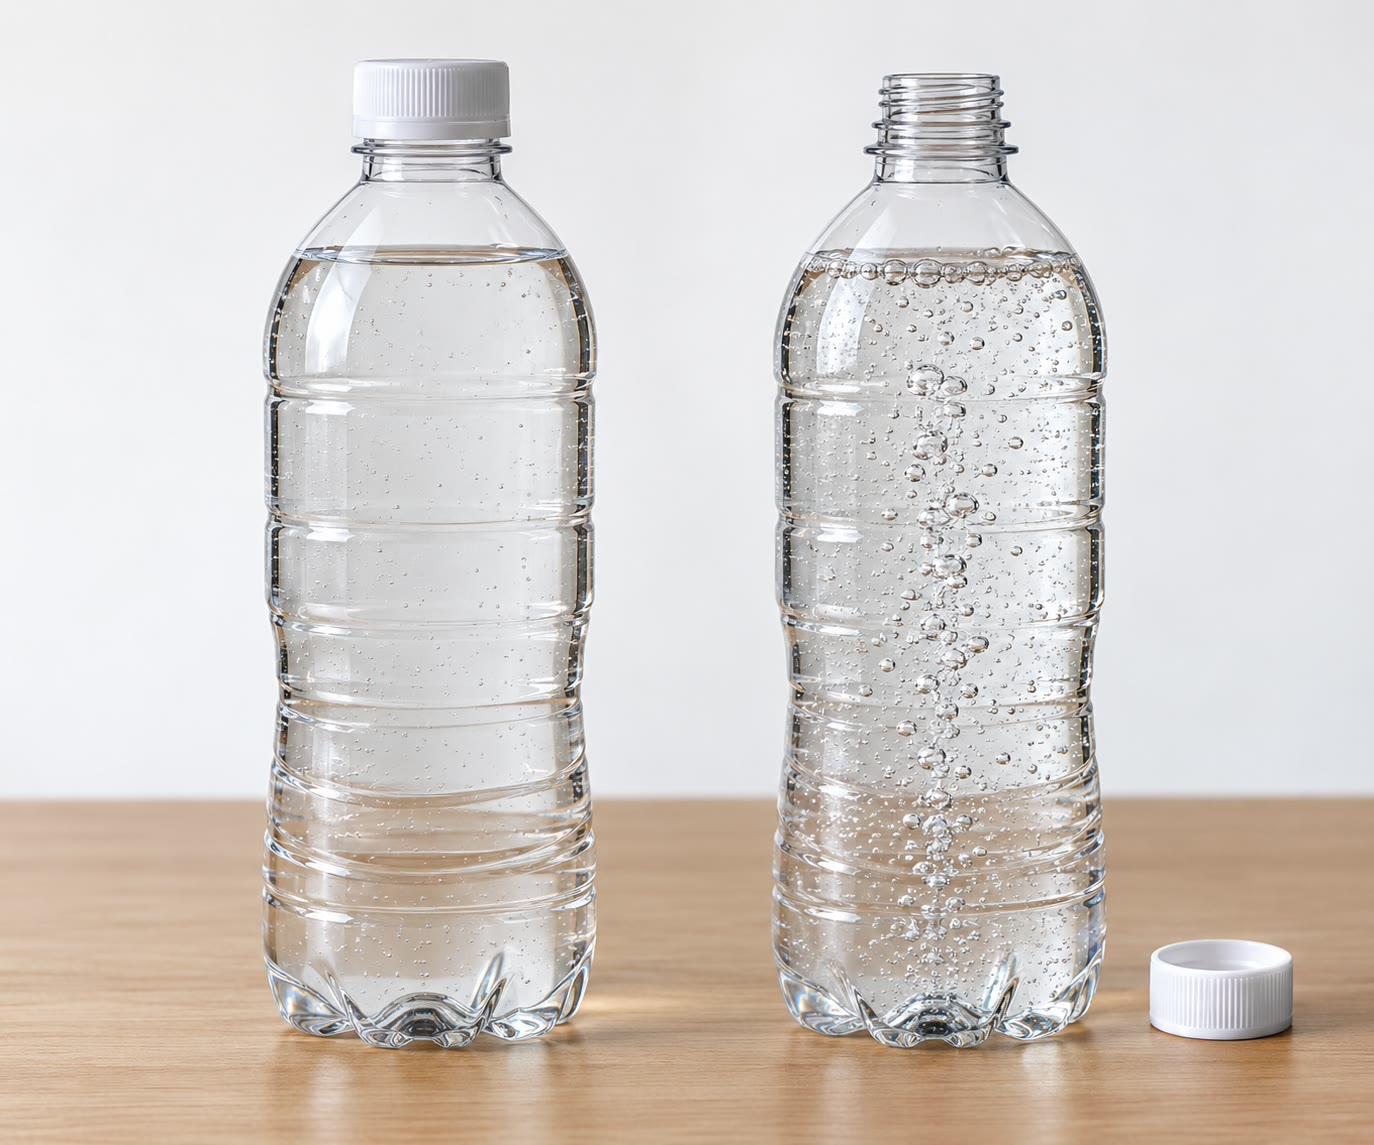
\includegraphics[width=0.45\linewidth,height=5cm,keepaspectratio]{images/book1/ai/g12-fizzy-bottles.jpg}

{\small Dicht houdt het water zijn gas; open ontsnapt het gas en komt het
niet terug.}
\end{omfigure}

\section{Reacties die niet aflopend zijn}

\begin{definition}[Niet-aflopende reactie, omzettingsgraad]\label{def:g12:equilibrium:non-total}
Een reactie is een \emph{niet-aflopende reactie}\index{niet-aflopende reactie}
als ze stopt bij een eindvoortgang $x_f$ die kleiner is dan haar
\omterm{def:g10:reaction-progress-table:limiting}{maximale voortgang} $x_{\max}$, terwijl alle \omterm{def:g7:chemical-reactions:reactant}{beginstoffen} nog aanwezig
zijn. Haar \emph{omzettingsgraad}\index{omzettingsgraad} is
\[
  \tau = \frac{x_f}{x_{\max}}, \qquad 0 < \tau < 1
\]
($\tau = 1$ bij een \omterm{def:g10:reaction-progress-table:limiting}{aflopende reactie}).
\end{definition}

\begin{example}[Een ester die halverwege stopt]\label{ex:g12:equilibrium:berthelot}
% ledger: ester:berthelot
Verwarmd met \qty{1}{mol} ethanol vormt \qty{1}{mol} ethaanzuur
ethylethanoaat en water,
\ce{CH3COOH + C2H5OH <=> CH3COOC2H5 + H2O}. De reactie stopt als ongeveer
twee derde van het zuur heeft gereageerd: $x_f = \qty{0.67}{mol}$ bij
$x_{\max} = \qty{1}{mol}$, dus $\tau \approx 0.67$. Uitgaande van
\qty{1}{mol} \omterm{def:g11:functional-groups:carboxylic-acid}{ester} en \qty{1}{mol} water stopt ook de omgekeerde reactie,
als ongeveer een derde van de \omterm{def:g11:functional-groups:carboxylic-acid}{ester} gehydrolyseerd is: hetzelfde
eindmengsel.
\end{example}

\begin{history}[Berthelot en Péan de Saint-Gilles, 1862]
% ledger: ester:berthelot
De scheikundigen Marcellin Berthelot en Léon Péan de Saint-Gilles
verwarmden \omterm{def:g6:pure-substances-and-mixtures:mixture}{mengsels} van ethaanzuur en ethanol, en van ethylethanoaat en
water, gedurende lange tijd, en analyseerden ze. Uitgaande van gelijke
hoeveelheden zuur en \omterm{def:g11:functional-groups:alcohol}{alcohol} stopte de reactie altijd bij ongeveer twee
derde; uitgaande van \omterm{def:g11:functional-groups:carboxylic-acid}{ester} en water bij een derde hydrolyse; en ze zagen
dat de hoeveelheid \omterm{def:g11:functional-groups:carboxylic-acid}{ester} die op elk moment ontstond, afhing van het
product van de hoeveelheden van de \omterm{def:g7:chemical-reactions:reactant}{beginstoffen}. Hun werk was een van de
eerste kwantitatieve studies van een chemisch evenwicht.
\end{history}

\section{De evenwichtstoestand}

\begin{definition}[Evenwichtstoestand]\label{def:g12:equilibrium:equilibrium-state}
Een systeem is in een \emph{evenwichtstoestand}\index{evenwichtstoestand}
als zijn samenstelling niet meer verandert, hoewel de heengaande en de
teruggaande reactie allebei nog doorgaan, met dezelfde snelheid. Een
reactie die zo'n toestand kan bereiken, schrijf je met de dubbele pijl
$\rightleftharpoons$.
\end{definition}

\begin{omfigure}
\begin{tikzpicture}
\begin{axis}[width=0.8\linewidth, height=6cm, xmin=0, xmax=200, ymin=0,
    ymax=1.05, xlabel={$t$ (\si{h})}, ylabel={hoeveelheid ester (\si{mol})},
    axis lines*=left, ymajorgrids, grid style={gray!20},
    tick label style={font=\small}, label style={font=\small},
    legend style={font=\small, at={(0.98,0.98)}, anchor=north east,
    draw=none, fill=white}, legend cell align=left]
  % ledger: ester:berthelot (K = 4; kinetics synthetic)
  \addplot[very thick, omDef] table[x=t, y=fromAcid] {figdata/out/grade-12-equilibrium.dat};
  \addplot[very thick, omProp] table[x=t, y=fromEster] {figdata/out/grade-12-equilibrium.dat};
  \addplot[dashed, black!60] coordinates {(0,0.6667) (200,0.6667)};
  \legend{uit 1 mol zuur + 1 mol alcohol, uit 1 mol ester + 1 mol water}
  \node[font=\small, anchor=north east] at (axis cs:195,0.65) {evenwicht: $\tfrac{2}{3}$ mol};
\end{axis}
\end{tikzpicture}

{\small De verestering (blauw) en de hydrolyse van de \omterm{def:g11:functional-groups:carboxylic-acid}{ester} (oranje)
bereiken dezelfde evenwichtssamenstelling, van tegengestelde kanten.
(De tijdschaal is een model; de eindwaarde is de gemeten waarde.)}
\end{omfigure}

\section{Het reactiequotiënt}

\begin{notation}[Standaardconcentratie]\label{not:g12:equilibrium:c-standard}
$c^\circ = \qty{1}{mol/L}$ is de standaardconcentratie. Een concentratie
delen door $c^\circ$ geeft een getal zonder eenheid met dezelfde waarde:
$[\ce{A}]/c^\circ$.
\end{notation}

\begin{definition}[Reactiequotiënt]\label{def:g12:equilibrium:quotient}
Voor een reactie in oplossing $a\,\ce{A} + b\,\ce{B} \rightleftharpoons c\,\ce{C} + d\,\ce{D}$ is het
\emph{reactiequotiënt}\index{reactiequotiënt} in een gegeven toestand van
het systeem
\[
  Q = \frac{\left([\ce{C}]/c^\circ\right)^c \left([\ce{D}]/c^\circ\right)^d}
           {\left([\ce{A}]/c^\circ\right)^a \left([\ce{B}]/c^\circ\right)^b} .
\]
Vaste stoffen, en het \omterm{def:g6:solutions-and-solubility:solute}{oplosmiddel} (water in een \omterm{def:g6:solutions-and-solubility:solute}{waterige oplossing}), komen
niet voor in $Q$.
\end{definition}


\begin{example}[Quotiënten opschrijven]\label{ex:g12:equilibrium:quotients}
Voor \ce{CH3COOH + H2O <=> CH3COO- + H3O+} in water (het \omterm{def:g9:ions:ion}{ion} \ce{H3O+}
wordt in het volgende hoofdstuk ingevoerd) is water het \omterm{def:g6:solutions-and-solubility:solute}{oplosmiddel}:
$Q = \dfrac{[\ce{CH3COO-}]\,[\ce{H3O+}]}{[\ce{CH3COOH}]\,c^\circ}$. Bij het
\omterm{def:g2:mixing-and-dissolving:dissolve}{oplossen} van een vaste stof, \ce{AgCl(s) <=> Ag+ + Cl-}, blijft de vaste
stof weg:
$Q = [\ce{Ag+}][\ce{Cl-}]/(c^\circ)^2$. Bij de verestering, waar alle vier
de deeltjes in hetzelfde vloeibare \omterm{def:g6:pure-substances-and-mixtures:mixture}{mengsel} met volume $V$ zitten, vallen de
volumes weg en geldt $Q = \dfrac{n_{\text{ester}}\, n_{\text{water}}}{n_{\text{zuur}}\, n_{\text{alcohol}}}$.
\end{example}

\section{De evenwichtsconstante}

\begin{definition}[Evenwichtsconstante]\label{def:g12:equilibrium:constant}
De waarde $Q_{eq}$ van het \omterm{def:g12:equilibrium:quotient}{reactiequotiënt} in de \omterm{def:g12:equilibrium:equilibrium-state}{evenwichtstoestand} is de
\emph{evenwichtsconstante}\index{evenwichtsconstante} $K$ van de reactie.
Ze heeft geen eenheid.
\end{definition}

\begin{proposition}[$K$ hangt alleen af van de temperatuur]\label{prop:g12:equilibrium:constant}
Voor een gegeven reactie is bij een gegeven temperatuur $Q_{eq} = K$ in
elke \omterm{def:g12:equilibrium:equilibrium-state}{evenwichtstoestand}, wat de beginhoeveelheden ook zijn.
\end{proposition}

\begin{proof}
Aangenomen; het wordt afgeleid in het deel voor het tweede
universiteitsjaar. Je kunt het controleren aan de verestering: beide
proeven in de figuur, gestart van tegengestelde kanten, geven dezelfde
$Q_{eq}$.
\end{proof}

\begin{example}[$K$ van de verestering]\label{ex:g12:equilibrium:k-ester}
% ledger: ester:berthelot
Uitgaande van \qty{1}{mol} zuur en \qty{1}{mol} \omterm{def:g11:functional-groups:alcohol}{alcohol} bevat het
evenwicht $\frac{2}{3}$ \omterm{def:g10:the-mole:amount}{mol} \omterm{def:g11:functional-groups:carboxylic-acid}{ester} en water en $\frac{1}{3}$ \omterm{def:g10:the-mole:amount}{mol} zuur en
\omterm{def:g11:functional-groups:alcohol}{alcohol}:
\[
  K = \frac{(2/3)\times(2/3)}{(1/3)\times(1/3)} = 4 .
\]
\end{example}

\begin{method}[Eindtoestand van een niet-aflopende reactie]\label{met:g12:equilibrium:final}
\begin{enumerate}
  \item Vul de \omterm{def:g10:reaction-progress-table:extent}{voortgangstabel} in met de onbekende eindvoortgang $x_f$.
  \item Schrijf $Q_{eq}$ als functie van $x_f$ en stel die gelijk aan $K$.
  \item Los $x_f$ op (vaak een vierkantsvergelijking) en houd de wortel
        tussen 0 en $x_{\max}$.
  \item Leid de eindhoeveelheden af en $\tau = x_f/x_{\max}$.
\end{enumerate}
\end{method}

\begin{example}[Een overmaat alcohol]\label{ex:g12:equilibrium:excess}
Uitgaande van \qty{1}{mol} zuur en \qty{2}{mol} \omterm{def:g11:functional-groups:alcohol}{alcohol} wordt de voorwaarde
voor het evenwicht $\dfrac{x^2}{(1-x)(2-x)} = 4$, dat is $3x^2 - 12x + 8 = 0$, waarvan de
wortel tussen 0 en 1 gelijk is aan $x_f = \qty{0.845}{mol}$. Een
verdubbeling van de \omterm{def:g11:functional-groups:alcohol}{alcohol} verhoogt het \omterm{def:g10:synthesis-yield:yield}{rendement}, gerekend op het zuur,
van \qty{67}{\percent} tot
\qty{85}{\percent}.
\end{example}

\section{De verandering voorspellen en verschuiven}

\begin{proposition}[Richting van de verandering]\label{prop:g12:equilibrium:direction}
Als $Q < K$, verandert het systeem in de heengaande richting (de
\omterm{def:g7:chemical-reactions:reactant}{reactieproducten} nemen toe) tot $Q = K$; als $Q > K$, verandert het in de
teruggaande richting; als $Q = K$, is het in evenwicht en verandert het
niet.
\end{proposition}

\begin{proof}
Aangenomen: $Q$ neemt toe als de heengaande reactie verloopt (de
\omterm{def:g7:chemical-reactions:reactant}{reactieproducten} in de teller nemen toe, de \omterm{def:g7:chemical-reactions:reactant}{beginstoffen} in de noemer
nemen af), en het systeem beweegt naar de toestand waarin $Q = K$.
\end{proof}

\begin{omfigure}
\begin{tikzpicture}[font=\small]
  \draw[->, thick] (0,0) -- (10,0) node[right] {$Q$};
  \draw[thick] (0,-0.12) -- (0,0.12) node[above] {0};
  \draw[very thick, omThm] (5,-0.25) -- (5,0.25) node[above] {$K$};
  \draw[->, very thick, omDef] (1.2,0.55) -- (4.4,0.55);
  \node[omDef, align=center] at (2.8,1.15) {$Q < K$: heen};
  \draw[->, very thick, omProp] (8.8,0.55) -- (5.6,0.55);
  \node[omProp, align=center] at (7.2,1.15) {$Q > K$: terug};
  \node[align=center] at (5,-0.75) {$Q = K$: evenwicht};
\end{tikzpicture}

{\small Het quotiënt beweegt altijd naar de constante toe.}
\end{omfigure}

\begin{remark}[Een evenwicht verschuiven]\label{rem:g12:equilibrium:shift}
Om meer product te krijgen uit een \omterm{def:g12:equilibrium:non-total}{niet-aflopende reactie}, kun je een
overmaat van een \omterm{def:g7:chemical-reactions:reactant}{beginstof} toevoegen (de goedkoopste), of een
\omterm{def:g7:chemical-reactions:reactant}{reactieproduct} weghalen zodra het ontstaat: allebei maken ze weer
$Q < K$, en het systeem schuift op in de heengaande richting. Het water
van een verestering weghalen (met een droogmiddel, of door het af te
destilleren) kan de reactie bijna tot het eind drijven. De geopende fles
bruisend water doet hetzelfde met het koolstofdioxide dat ontsnapt.
\end{remark}

\begin{omfigure}
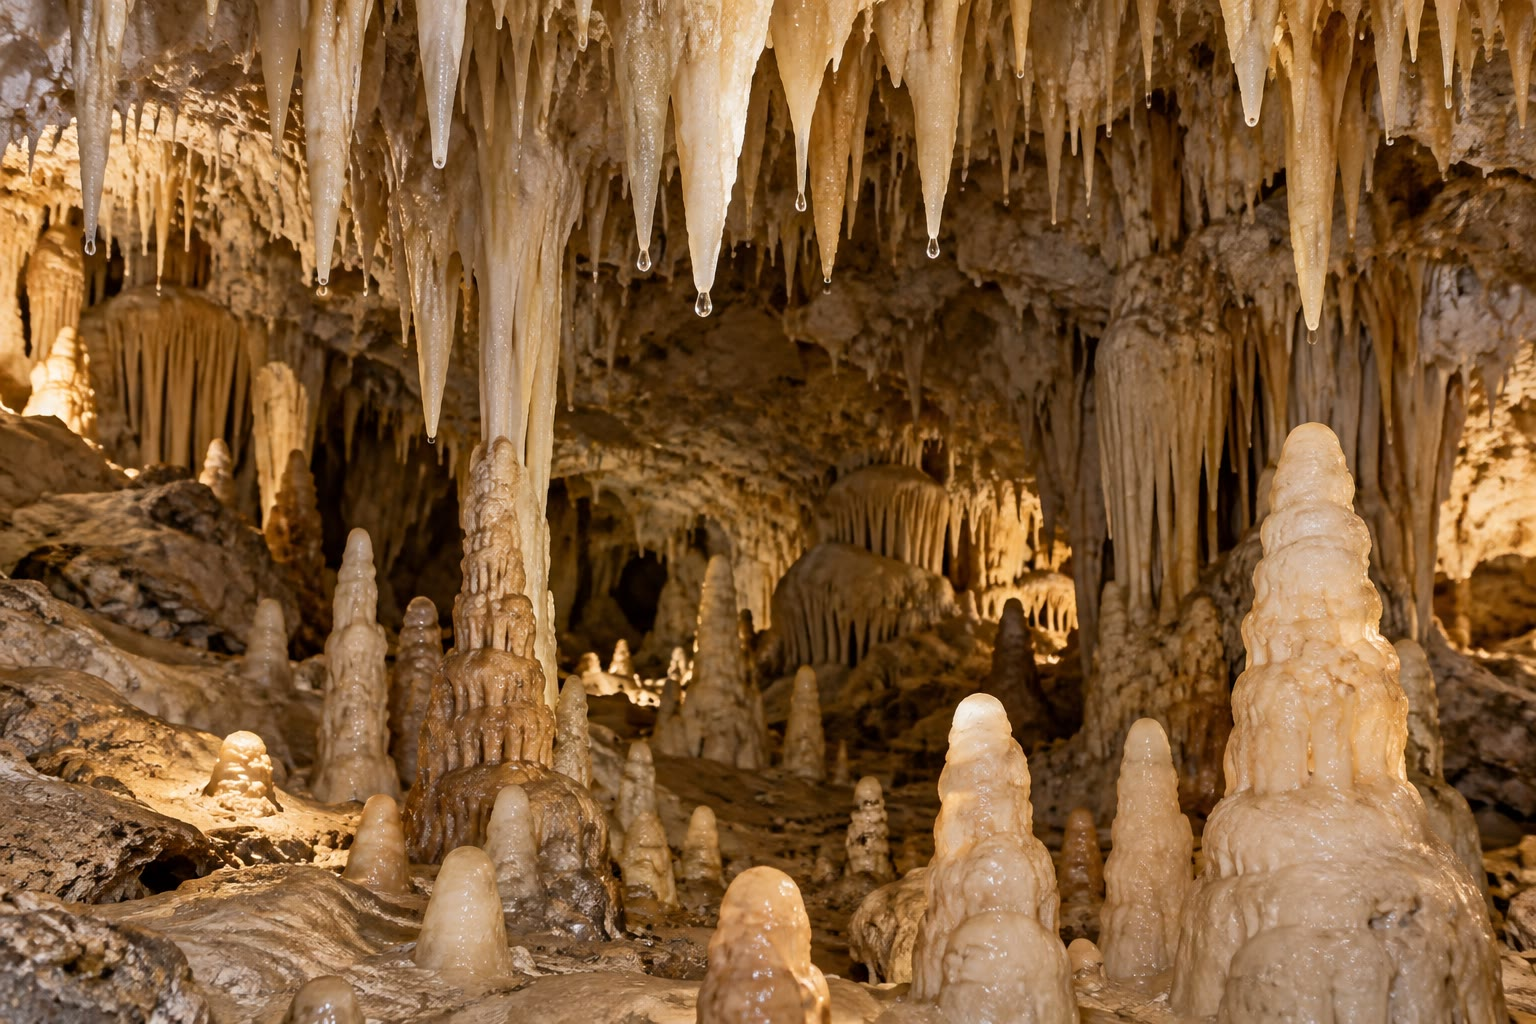
\includegraphics[width=0.45\linewidth]{images/book1/ai/g12-cave-stalactites.jpg}

{\small Stalactieten groeien waar water dat in een grot druppelt,
koolstofdioxide aan de \omterm{def:g4:air-a-mixture-of-gases:air}{lucht} verliest: een evenwicht van opgeloste
kalksteen verschuift, en er slaat calciumcarbonaat neer.}
\end{omfigure}

\section{Oefeningen}

\begin{exercise}[$\star$]\label{exo:g12:equilibrium:1}
Schrijf het \omterm{def:g12:equilibrium:quotient}{reactiequotiënt} op van: (a) \ce{N2 + 3H2 <=> 2NH3} (gassen,
gebruik concentraties); (b) \ce{CH3COOH + H2O <=> CH3COO- + H3O+} in
water;
(c) \ce{CaCO3(s) <=> Ca^{2+} + CO3^{2-}}; (d) \ce{Fe^{3+} + SCN- <=>
FeSCN^{2+}}.
\end{exercise}

\begin{exercise}[$\star$]\label{exo:g12:equilibrium:2}
Een reactie heeft $x_{\max} = \qty{0.050}{mol}$ en bereikt
$x_f = \qty{0.020}{mol}$. Bereken $\tau$. Is de reactie aflopend?
\end{exercise}

\begin{exercise}[$\star$]\label{exo:g12:equilibrium:3}
In welke richting verandert een \omterm{def:g6:pure-substances-and-mixtures:mixture}{mengsel} bij een reactie met $K = 10$ als
$Q = 2$? Als $Q = 50$? Als $Q = 10$?
\end{exercise}

\begin{exercise}[$\star$]\label{exo:g12:equilibrium:4}
Leg uit waarom een evenwicht ``dynamisch'' heet.
\end{exercise}

\begin{exercise}[$\star$]\label{exo:g12:equilibrium:5}
Verandert een \omterm{def:g12:catalysis:catalyst}{katalysator} $K$? De tijd die nodig is om het evenwicht te
bereiken? Leg uit.
\end{exercise}

\begin{exercise}[$\star\star$]\label{exo:g12:equilibrium:6}
\qty{2.0}{mol} ethaanzuur en \qty{2.0}{mol} ethanol worden gemengd
($K = 4$). Bereken de eindhoeveelheden van de vier deeltjes.
\end{exercise}

\begin{exercise}[$\star\star$]\label{exo:g12:equilibrium:7}
Een \omterm{def:g6:pure-substances-and-mixtures:mixture}{mengsel} bevat van elk \qty{0.5}{mol}: ethaanzuur, ethanol,
ethylethanoaat en water. Bereken $Q$. In welke richting verandert het?
\end{exercise}

\begin{exercise}[$\star\star$]\label{exo:g12:equilibrium:8}
Lees in de figuur van de twee proeven de hoeveelheid \omterm{def:g11:functional-groups:carboxylic-acid}{ester} na
\qty{20}{h} in elke proef af. Wanneer kun je het systeem als in evenwicht
beschouwen?
\end{exercise}

\begin{exercise}[$\star\star$]\label{exo:g12:equilibrium:9}
Bereken met de methode van het hoofdstuk de eindhoeveelheden uitgaande van
\qty{1}{mol} \omterm{def:g11:functional-groups:carboxylic-acid}{ester} en \qty{1}{mol} water ($K = 4$ voor de verestering,
dus $1/4$ voor de hydrolyse), en vergelijk met de proef van de
verestering.
\end{exercise}

\begin{exercise}[$\star\star$]\label{exo:g12:equilibrium:10}
Waarom staat de vaste stof niet in het quotiënt van
\ce{AgCl(s) <=> Ag+ + Cl-}? Verschuift het evenwicht als je meer vaste
stof toevoegt?
\end{exercise}

\begin{exercise}[$\star\star$]\label{exo:g12:equilibrium:11}
In een dichte fles bruisend water verlaat koolstofdioxide het water en
komt het erin terug met dezelfde snelheid. Schrijf het evenwicht
\ce{CO2(aq) <=> CO2(g)} op en leg met $Q$ en $K$ uit waarom het water zijn
prik verliest als de fles geopend wordt.
\end{exercise}

\begin{exercise}[$\star\star\star$]\label{exo:g12:equilibrium:12}
Een verestering van \qty{1}{mol} zuur en \qty{1}{mol} \omterm{def:g11:functional-groups:alcohol}{alcohol} bereikt het
evenwicht. Daarna wordt de helft van het aanwezige water weggehaald.
Bereken de nieuwe $Q$, zeg in welke richting het systeem verandert, en
bepaal de nieuwe eindhoeveelheid \omterm{def:g11:functional-groups:carboxylic-acid}{ester}.
\end{exercise}

\begin{exercise}[$\star\star\star$]\label{exo:g12:equilibrium:13}
Laat zien dat de constante van de omgekeerde reactie $1/K$ is. Wat is de
constante van de hydrolyse van ethylethanoaat?
\end{exercise}

\begin{exercise}[$\star\star\star$]\label{exo:g12:equilibrium:14}
Een scheikundige \omterm{def:g2:mixing-and-dissolving:mix}{mengt} \qty{1}{mol} zuur, \qty{1}{mol} \omterm{def:g11:functional-groups:alcohol}{alcohol},
\qty{2}{mol} \omterm{def:g11:functional-groups:carboxylic-acid}{ester} en \qty{0.5}{mol} water. Gebeurt er iets? Leg uit.
\end{exercise}

\begin{exercise}[$\star\star\star$]\label{exo:g12:equilibrium:15}
Welke overmaat \omterm{def:g11:functional-groups:alcohol}{alcohol} (hoeveelheid per \omterm{def:g10:the-mole:amount}{mol} zuur) is er nodig om
\qty{95}{\percent} van het zuur te veresteren? Los
$\dfrac{0.95^2}{0.05(n - 0.95)} =
4$ op.
\end{exercise}

\section{Probleem: De ester van Berthelot}

\begin{problem}[{Weekendprobleem --- hoeveel ester als de alcohol in
drievoudige overmaat wordt toegevoegd?}]
\label{pb:g12:equilibrium:1}
% ledger: ester:berthelot, aw:C, aw:H, aw:O
Ethylethanoaat, een \omterm{def:g6:solutions-and-solubility:solute}{oplosmiddel} en een smaakstof, wordt gemaakt uit
ethaanzuur en ethanol. In 1862 vonden Berthelot en Péan de Saint-Gilles
dat de reactie, uitgaande van gelijke hoeveelheden zuur en \omterm{def:g11:functional-groups:alcohol}{alcohol}, stopt
als ongeveer twee derde van het zuur heeft gereageerd.

\medskip
\noindent\textbf{Deel I --- De reactie.}
\begin{enumerate}
  \item Schrijf de vergelijking van de verestering op, met \omterm{def:g11:organic-skeletons:formulas}{beknopte
        structuurformules}.
  \item Waarom wordt ze met een dubbele pijl geschreven?
  \item Schrijf haar \omterm{def:g12:equilibrium:quotient}{reactiequotiënt} op in hoeveelheden.
  \item Wat is $x_{\max}$, uitgaande van \qty{1}{mol} zuur en
        \qty{1}{mol} \omterm{def:g11:functional-groups:alcohol}{alcohol}? Wat is $x_f$, volgens het resultaat van
        Berthelot?
  \item Bereken $\tau$.
\end{enumerate}

\medskip
\noindent\textbf{Deel II --- De constante.}
\begin{enumerate}[resume]
  \item Geef de eindhoeveelheden van de vier deeltjes.
  \item Bereken $K$.
  \item Uitgaande van \qty{1}{mol} \omterm{def:g11:functional-groups:carboxylic-acid}{ester} en \qty{1}{mol} water vond
        Berthelot een derde gehydrolyseerd. Laat zien dat dit klopt met
        dezelfde $K$.
  \item Waarom moet $K$ in beide gevallen dezelfde zijn?
\end{enumerate}

\medskip
\noindent\textbf{Deel III --- Een drievoudige overmaat \omterm{def:g11:functional-groups:alcohol}{alcohol}.}
\begin{enumerate}[resume]
  \item Vul de \omterm{def:g10:reaction-progress-table:extent}{voortgangstabel} in, uitgaande van \qty{1}{mol} zuur en
        \qty{3}{mol} \omterm{def:g11:functional-groups:alcohol}{alcohol}.
  \item Schrijf de vergelijking $Q_{eq} = K$ op en laat zien dat ze
        $3x^2 - 16x + 12 = 0$ wordt.
  \item Los haar op, en houd de zinvolle wortel.
  \item Welk deel van het zuur wordt veresterd?
  \item Bereken de massa \omterm{def:g11:functional-groups:carboxylic-acid}{ester} die je krijgt.
\end{enumerate}

\medskip
\noindent\textbf{Deel IV --- Water weghalen.}
\begin{enumerate}[resume]
  \item Uitgaande van het equimolaire evenwicht wordt het water
        weggehaald zodra het ontstaat. Leg met $Q$ uit waarom de reactie
        doorgaat.
  \item Wat zou het \omterm{def:g10:synthesis-yield:yield}{rendement} worden als al het water weggehaald kon
        worden?
  \item Waarom wordt meestal de \omterm{def:g11:functional-groups:alcohol}{alcohol}, en niet het zuur, in overmaat
        toegevoegd? (Denk aan de kosten en aan het scheiden van de
        producten.)
  \item Verandert verwarmen van het \omterm{def:g6:pure-substances-and-mixtures:mixture}{mengsel} de \omterm{def:g10:reaction-progress-table:system}{eindtoestand}, of alleen de
        tijd om die te bereiken? (Bij de verestering komt bijna geen
        warmte vrij.)
  \item Geef het eindantwoord: welk deel van het zuur wordt veresterd bij
        een drievoudige overmaat \omterm{def:g11:functional-groups:alcohol}{alcohol}?
\end{enumerate}
\end{problem}
